%----------------DEFINE FORMA CORRETA DE HIFENIZAÇÃO PARA ALGUMAS PALAVRAS ----------------
\hyphenation{am-bi-en-te}
\hyphenation{res-pos-ta}
\hyphenation{res-pos-tas}
\hyphenation{exis-tem}
\hyphenation{va-lor}
\hyphenation{va-lo-res}
\hyphenation{im-pe-ra-ti-va}
\hyphenation{im-pe-ra-ti-vas}
\hyphenation{im-pe-ra-ti-vo}
\hyphenation{im-pe-ra-ti-vos}
\hyphenation{ou-tra}
\hyphenation{ou-tro}
\hyphenation{ou-tras}
\hyphenation{ou-tros}
\hyphenation{pro-ble-ma}
\hyphenation{res-tri-to}
\hyphenation{res-tri-tos}
\hyphenation{res-tri-ta}
\hyphenation{res-tri-tas}
\hyphenation{me-lho-rar}
\hyphenation{fun-cio-na-li-da-de}
\hyphenation{fun-cio-na-li-da-des}
\hyphenation{apre-sen-ta-do}
\hyphenation{mo-de-lo}
\hyphenation{apre-sen-ta-dos}
\hyphenation{apre-sen-ta-da}
\hyphenation{apre-sen-ta-das}
\hyphenation{do-cu-men-to}
\hyphenation{LuaSQL}
\hyphenation{e-co-no-mi-zar}
%\hyphenation{ca-rac-te-rís-ti-ca}
%\hyphenation{ca-rac-te-rís-ti-cas}
%----------------DEFINE FORMA CORRETA DE HIFENIZAÇÃO PARA ALGUMAS PALAVRAS ----------------

Um dos grandes atrativos da TV Digital (TVD) é com certeza a interatividade. 
O nível de interatividade das aplicações vai desde a chamada interatividade local
(onde os usuários podem acessar apenas os dados enviados pela emissora)
até a interatividade plena (onde os usuários dispõem de um canal de retorno, permitindo
enviar e receber dados em uma rede como a \textit{Internet}) \cite{soares2009programando}. 

As aplicações com interatividade plena precisam utilizar protocolos de comunicação 
padrões (como TCP, HTTP e SOAP) para garantir a interoperabilidade
com outros sistemas. Utilizando os protocolos citados, é possível garantir a convergência entre \textit{Web} e TV.
Com isto, as aplicações de TVDi podem ser enriquecidas com conteúdo proveniente da \textit{Internet},
como o projeto apresentado em \cite{socialnets-tvd2010ghisi}.

No entanto, a norma do sub-sistema Ginga-NCL do \textit{middleware} Ginga define 
apenas a obrigatoriedade do protocolo TCP. Quaisquer protocolos acima da camada de transporte
precisam ser implementados pelo desenvolvedor de aplicações. 

Assim, são apresentados neste artigo os projetos NCLua HTTP e NCLua SOAP: módulos Lua que implementam HTTP e SOAP para o sub-sistema Ginga-NCL.
O desenvolvimento dos projetos partiu da inexistência de versões livres e de código aberto de tais protocolos para o Ginga-NCL.

O artigo está organizado como segue. Na Seção \ref{sec:problema} é apresentado o problema de consumo de \textit{Web Services} em aplicações
para o Ginga-NCL; na Seção \ref{sec:trabs-rel} as tecnologias e trabalhos relacionados;
na Seção \ref{sec:modulos-implementados} os módulos implementadas; 
na Seção \ref{sec:resultados} os resultados alcançados e exemplos de utilização;
na Seção \ref{sec:conclusao} as conclusões e por fim os trabalhos futuros.

\section{Delimitação do Problema} \label{sec:problema}

Apesar de Lua ser uma linguagem extensível \cite{ierusalimschy2007evolution}, principalmente pela capacidade de utilizar módulos construídos em linguagem C, e de existirem vários destes módulos para as mais diversas finalidades, tais módulos binários não podem ser utilizados em aplicações de TVDi enviadas via \textit{broadcast}, devido a questões de segurança, uma vez que um módulo escrito em linguagem C pode ter acesso a qualquer funcionalidade do sistema operacional (embarcado com o \textit{middleware} no receptor de TVD). 

Em \cite{braga-introducao} são citadas algumas ameaças de segurança em sistemas de TVDi, como 
transações fraudulentas, pirataria de conteúdo, entre outras. Tais ameaças podem ser potencializadas com o uso de módulos binários. Além do mais, módulos em C possuem código nativo dependente de plataforma, o que não garante que a aplicação executará em qualquer receptor \cite{costa-seguranca}.
Somente aplicações residentes podem ser desenvolvidas em linguagens compiladas como C.

Com isto, para haver, em aplicações NCLua de TVDi, algumas das funcionalidades dos módulos binários citados, é preciso
implementar módulos inteiramente em linguagem Lua, cujo ciclo de vida é controlado pelo \textit{middleware} Ginga\cite{abnt200815606}.

\section{Trabalhos Relacionados} \label{sec:trabs-rel}

A seguir são apresentadas as tecnologias envolvidas na solução
proposta e os trabalhos relacionados.

\subsection{Lua e os \textit{scripts} NCLua} \label{sec:lua-nclua}

Lua é a linguagem imperativa utilizada pelo sub-sistema Ginga-NCL para o desenvolvimento
de aplicações procedurais. 

Como a linguagem NCL é apenas declarativa, a inclusão de características imperativas
a uma aplicação de TVDi para o Ginga-NCL é possibilitada por meio dos chamados
NCLua, \textit{scripts} Lua funcionando como nós de mídia dentro de um documento NCL 
\cite{abnt200815606} \cite{soares2007ginga}. 
O que diferencia os \textit{scripts} NCLua de \textit{scripts} Lua convencionais é a possibilidade de comunicação
bidirecional, por meio de eventos, entre este e o documento NCL \cite{abnt200815606}.

O tratamento de eventos e as particularidades associadas a aplicações Lua para TVDi
são implementadas por módulos adicionais à Linguagem\cite{abnt200815606}.
Os módulos de NCLua utilizados no presente artigo são: \textbf{\textit{event}}, 
para comunicação bidirecional entre um NCL e um NCLua;
e \textbf{\textit{canvas}}, para desenhar imagens e primitivas gráficas.

\subsection{Protocolo TCP no Ginga-NCL} \label{sec:tcp}

A norma do Ginga-NCL \cite{abnt200815606} define a disponibilidade do protocolo TCP
por meio da classe de eventos \textit{tcp} do módulo \textit{event}. 
Este permite o tratamento de eventos e a comunicação assíncrona entre o formatador NCL e os \textit{scripts} NCLua. 

Devido à característica assíncrona do módulo \textit{event}, o tratamento de requisições TCP em NCLua não é trivial,
necessitando do uso de co-rotinas da linguagem Lua, como implementado no módulo \textit{tcp.lua} em \cite{doc-nclua}. 
Co-rotinas são similares a um \textit{thread} \cite{ierusalimschy2006programming}.

A Figura \ref{fig:tcp-state-machine} apresenta um gráfico de máquinas de estados
da realização de uma conexão TCP no Ginga-NCL, utilizando o módulo \textit{tcp.lua}.
A aplicação estabelece uma conexão a um servidor, envia uma requisição e fica aguardando o retorno. 
A função \textit{tcp.receive} é executada até que não hajam mais dados a receber, 
realizando a desconexão.

\begin{center}
	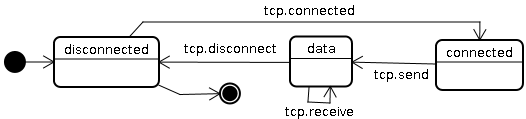
\includegraphics[scale=0.4]{ncluasoap-Statemachine-TCP.png}
	\captionof{figure}{Diagrama de Máquinas de Estados do Módulo \textit{tcp.lua}}
	\label{fig:tcp-state-machine}
\end{center}

A Figura \ref{fig:tcp-state-machine-coroutines} apresenta um gráfico do ponto de vista das co-rotinas em execução. 
O módulo inicia criando uma co-rotina. A função \textit{coroutine.resume}
inicia a execução da co-rotina. Quando é solicitada uma tentativa de
conexão, a co-rotina é suspensa (aguardando até uma conexão ser estabelecida).
Após a conexão, a co-rotina é novamente resumida (continuando a execução),
permitindo que seja enviada uma requisição ao servidor (\textit{tcp.send}). 
Para a obtenção da resposta da requisição,  
usa-se a função \textit{tcp.receive}, suspendendo a co-rotina
novamente, até que algum dado seja obtido.

\begin{center}
	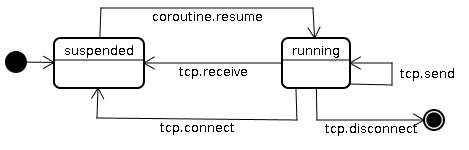
\includegraphics[scale=0.4]{ncluasoap-Statemachine-TCP-Coroutines.png}
	\captionof{figure}{Diagrama de Máquinas de Estados do Módulo \textit{tcp.lua} (corotinas em execução)}
	\label{fig:tcp-state-machine-coroutines}
\end{center}

A implementação realizadas simplificam diversas chamadas de funções e co-rotinas necessárias à realização de uma conexão TCP no Ginga-NCL,
encapsulando diversos detalhes deste processo.

\subsection{Implementações de SOAP}

SOAP é um protocolo do \textit{World Wide Web Consortium} (W3C), baseado em XML, que permite a aplicações disponibilizarem serviços na \textit{Web}, em uma arquitetura distribuída no modelo cliente/servidor. 
Tais serviços, denominados \textit{Web Services} (WS), podem ser providos e consumidos por aplicações desenvolvidas em diferentes linguagens e plataformas
\cite{soap-spec} \cite{curbera2002unraveling} \cite{newcomer2002understanding}.
O protocolo possui uma linguagem para descrição dos serviços disponibilizados, a \textit{Web Service Description Language} (WSDL).
De forma padronizada (manual ou automatizadamente), uma aplicação cliente pode conhecer os serviços
de um \textit{Web Service} lendo o WSDL do mesmo\cite{soap-spec}.

A seguir são analisados alguns \textit{toolkits} para provimento e consumo de \textit{WS's} SOAP.

Para acesso a \textit{WS's} SOAP a partir de aplicações Lua, pode-se utilizar o módulo LuaSOAP \cite{luasoap}.
O projeto utiliza o \textit{Expat} \cite{expat}\cite{cooper1999using} para 
tratamento de XML. Este é um \textit{parser} XML desenvolvido em linguagem C, cujos problemas de uso
em aplicações de TVDi foram apresentados na Seção \ref{sec:problema}. Ele usa a biblioteca \textit{LuaSocket},
que depende de módulos em C. 
Uma das vantagens do projeto é que as chamadas aos métodos remotos no \textit{WS} são síncronas, o que facilita
bastante o uso.

O gSOAP é um projeto que permite a aplicações desenvolvidos em linguagens C, C++ ou Fortran,  
consumirem \textit{WS's}\cite{van2005gsoap}. O projeto possui um utilitário para gerar \textit{stubs} em C/C++, a partir do WSDL do serviço. Em tal \textit{stub} são incluídos métodos \textit{proxies} para realizar chamadas aos métodos remotos do serviço. 
Por ser desenvolvido em C, o mesmo só pode ser utilizado
em aplicações de TVD residentes.

Em \cite{davis2005latency} são apresentados outros \textit{toolkits} SOAP, como o Apache Axis, uma implementação de SOAP para Java e C. No entanto, esta não atende a um dos requisitos desejados: ser implementado em Lua para uso direto no Ginga-NCL.

%------------------------------------------------------------------------------------------------------------------------
\section{Proposta} \label{sec:modulos-implementados}

A seguir são apresentados os módulos implementados.
O NCLua SOAP está disponível em \url{http://ncluasoap.manoelcampos.com}. 
O NCLua HTTP está disponível em \url{http://ncluahttp.manoelcampos.com}. 
Tais URL's contêm os módulos, exemplos e toda a documentação dos mesmos.
Para montagem do ambiente de desenvolvimento e testes de aplicações que utilizem
os módulos implementados são necessários:
\begin{itemize}
	\item máquina virtual Ginga Virtual Set-top Box 0.12.1 rev 34 ou superior (a ser executada com o VMWare Player);
	\item IDE Eclipse 3.6.1 para criação de projetos de aplicações;
	\item plugin NCLEclipse 1.5.1 para dar suporte à linguagem NCL no Eclipse e poder transferir
	os arquivos das aplicações para a máquina virtual Ginga Virtual Set-top Box;
	\item plugin LuaEclipse 1.3.1 para dar suporte à linguagem Lua no Eclipse.
\end{itemize}

\subsection{NCLua HTTP} \label{sec:ncluahttp}

O NCLua HTTP implementa alguns dos principais recursos do protocolo HTTP/1.0. 
Ele é um módulo escrito inteiramente em linguagem Lua
para ser utilizado em \textit{scripts} NCLua. 
O mesmo utiliza o protocolo TCP da forma como especificado na norma \cite{abnt200815606}.

Pela simplicidade do protocolo HTTP, o módulo possui apenas algumas funções que permitem a geração
de requisições e tratamento de respostas. Atualmente existem os seguintes recursos implementados: 
autenticação básica; download de arquivos;
requisições \textit{GET} e \textit{POST};
passagem de cabeçalhos HTTP e definição de \textit{User-Agent};
separação automática dos dados do cabeçalho e do corpo da resposta de uma requisição.

\subsection{NCLua SOAP} \label{sec:ncluasoap}
O NCLua SOAP implementa as principais funcionalidades do protocolo SOAP 1.1 e 1.2. 
Ele também é um módulo inteiramente
escrito em Lua, que faz o \textit{parse} de arquivos XML, 
realizando o \textit{marshalling} e \textit{unmarshalling} de/para tabelas Lua, permitindo que o desenvolvedor Lua
trabalhe com a estrutura de dados principal da linguagem: o tipo \textit{table}.

O módulo utiliza o NCLua HTTP para transportar as mensagens SOAP. Com isto, a implementação do SOAP fica bastante simplificada, tornando o código
fácil de ser mantido. O NCLua SOAP encarrega-se apenas de gerar o XML da requisição SOAP, utilizando
o NCLua HTTP para enviar tal XML no corpo da mensagem. O \textit{parse} e \textit{unmarshalling} do XML para uma tabela Lua
é todo encapsulado pelo módulo LuaXML\footnote{\textit{Parser} XML escrito inteiramente em Lua, adaptado para funcionar com Lua 5}. 

Um importante recurso, que facilita bastante a utilização do módulo, é a simplificação 
do XML retornando como resposta, que é convertido (\textit{unmarshalling}) automaticamente para uma tabela Lua.
Para demonstrar este recurso, utilizar-se-á um \textit{WS} de consulta de endereço a partir de um CEP. 
Tal WS possui um método chamado "cep",
que recebe um determinado CEP e retorna o endereço referente ao mesmo.
O XML de retorno do método "cep", apresentado como tabela Lua, é semelhante ao da Listagem \ref{list:cepws}.

\begin{lstlisting}[caption=Tabela Lua gerada a partir de um XML de resposta a uma requisição SOAP, label=list:cepws, language=lua]
{cepResult =  {diffgr = {NewDataSet = {tbCEP = {
   nome="Cln 407", bairro="Asa Norte", UF="DF", cidade="Brasilia" }}}}}
\end{lstlisting}

Como pode ser visto, o elemento
da tabela que contém de fato os dados do endereço retornado (tbCEP) está envolvido em 
várias outras tabelas que não contém dado algum, sendo estruturas completamente
desnecessárias para a aplicação NCLua. Com isto, para o desenvolvedor
poder acessar, por exemplo, a cidade do CEP indicado, precisará 
conhecer toda a estrutura retornada, utilizando uma instrução como
\textit{result.cepResult.diffgr.NewDataSet.tbCEP.cidade}.

Para esconder estes detalhes do desenvolvedor, o NCLua SOAP simplifica qualquer
resultado que contenha estruturas desnecessárias, como o mostrado na Listagem \ref{list:cepws}.
Desta forma, para o exemplo citado, a tabela Lua (gerada a partir do XML de retorno da requisição) 
ficará como apresentado na Listagem \ref{list:ncluasoap-tb}, o que simplifica
o acesso aos elementos da estrutura retornada, permitindo, por exemplo, que o campo
cidade seja acessado utilizando-se apenas a instrução \textit{result.cidade}.

\begin{lstlisting}[caption=Simplificação de retorno de uma requisição SOAP feita pelo NCLua SOAP, label=list:ncluasoap-tb, language=lua]
{   nome="Cln 407", bairro="Asa Norte", UF="DF", cidade="Brasilia"   }
\end{lstlisting}

O módulo ainda possui um \textit{script} (\textit{wsdlparser.lua}) que realiza
o \textit{parse} de um WSDL e obtém algumas das informações que precisa-se
passar para que ele realize a requisição 
(como o \textit{namespace} do serviço e o nome do método desejado).

Para resumir, as características principais do NCLua SOAP são: suporte a SOAP 1.1 e 1.2;
parâmetros de entrada e saída \textit{struct} e \textit{array}; 
facilidade para manipular chamadas assíncronas;
simplicidade na obtenção do retorno de uma chamada remota;
SOAP \textit{Fault} para captura de erros SOAP;
SOAP \textit{Header}\cite{soap-spec} para passagem de parâmetros específicos da aplicação 
(como informações de autenticação, pagamento, etc).

A Figura \ref{fig:diagrama-componentes} apresenta um diagrama de componentes dos módulos implementados,
mostrando a dependência entre os componentes. Todos os módulos já foram
apresentados, exceto o \textit{NCLua HTTP Client App} e o \textit{NCLua SOAP Client App},
que representam, respectivamente, uma aplicação cliente usando HTTP e
uma aplicação consumindo \textit{WS's}.

\begin{center}
	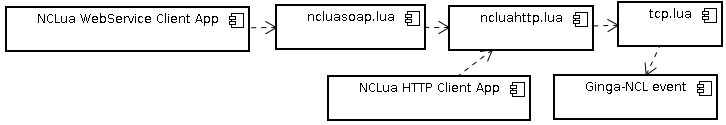
\includegraphics[width=1\textwidth]{ncluasoap-component-diagram.png}
	\captionof{figure}{Diagrama de Componentes do NCLua SOAP e NCLua HTTP}
	\label{fig:diagrama-componentes}
\end{center}

\section{Estudos de Caso} \label{sec:use-case}
\added{
As implementações apresentadas agilizam a construção de aplicações
com interatividade plena, realizando acesso ao canal de retorno
por meio de protocolos padronizados. Existem diversas categorias
de aplicações interativas que podem ser construídas
com uso dos protocolos implementados, 
tais como jogos, informações (notícias, horóscopo, previsão do tempo, etc), 
educação (\textit{T-Learning}), governo eletrônico (\textit{T-Government}), comércio eletrônico (\textit{T-Commerce}), 
saúde (\textit{T-Health}), bancárias (\textit{T-Banking}) e outras, como apresentado em \cite{fernandez2008aplicaciones},
\cite{de-usabilidade} e \cite{tgov2010barbosa}.
}

\added{
Dentre as categorias de aplicações apresentadas, as aplicações 
de governo eletrônico, saúde e educação pública tem como objetivo
fornecer serviços à população em geral, democratizando
e tornando mais acessíveis serviços que normalmente são disponibilizados
em sedes de órgãos do governo ou pela \textit{Internet}.
Com o uso dos recursos de interatividade da TV Digital, aplicações
destas categorias servem para promover a inclusão digital e social.
}

\added{
Alguns dos serviços que podem ser providos pela TV Digital são:
\begin{itemize}
 	\item marcação de consultas em hospitais públicos;
 	\item enquetes/consultas à população;
 	\item campanhas de vacinação e para controle de epidemias;
 	\item educação à distância, tutores inteligentes;
 	\item informações de previdência social (como o projeto TV Digital Social\footnote{\url{http://clube.ncl.org.br/node/101}})
 \end{itemize}  
}

\added{
Apesar de a TV estar em cerca de 96\% dos lares brasileiros\cite{ibge-pnad}, em 2009, 
apenas 25\% dos lares tinham acesso à Internet\cite{tic2009}. O uso da interatividade
plena requer acesso à \textit{Internet}, e como pôde-se ver, o acesso residencial
à mesma, no Brasil, é bastante restrito. No entanto, com a criação do 
Plano Nacional de Banda Larga (PNBL) por meio do Decreto número 7.175, de 12 de maio de 2010,
visando prover \textit{Internet} banda larga a um custo reduzido, este cenário tende a mudar.
Desta forma, o uso de serviços da \textit{Internet}, inclusive de governo eletrônico,
por meio de protocolos como HTTP e SOAP, se tornará cada vez mais popular, considerando
todos os benefícios de agilidade que estes trazem, sem a necessidade de locomoção
do cidadão até uma agência do governo.
}

\section{Resultados} \label{sec:resultados}

Foram realizados diversos testes de interoperabilidade com servidores
\textit{Web} e \textit{WS's}, estes últimos desenvolvidos
em diferentes linguagens. A atual versão dos módulos conseguiu
fazer a interoperação com tais serviços normalmente.
As subseções a seguir apresentam exemplos de uso dos módulos implementados.

\subsection{Exemplos de uso do NCLua HTTP}

O exemplo da Listagem \ref{list:ncluahttp2} envia uma requisição HTTP \textit{GET} para uma página
\textit{Web}, com o parâmetro "voto" igual a "sim", obtendo o resultado e exibindo no terminal. 

A linha 1 adiciona o módulo NCLua HTTP. 
A linha 7 chama a função \textit{http.request}
que envia a requisição HTTP. Devido à particularidade assíncrona
do protocolo TCP no Ginga-NCL (que é utilizado para transportar as mensagens HTTP), 
para facilitar o envio de requisições e recebimento de respostas,
o módulo NCLua HTTP utiliza co-rotinas de Lua. 
Por este motivo, a obtenção do retorno deve ser feita dentro de uma função, como
a definida na linha 5, contendo os parâmetros \textit{header} e \textit{body} (comentados na definição
da mesma). Tal função deve ser passada como parâmetro à \textit{http.request}, para que seja
chamada por esta quando a resposta for obtida. 

\begin{lstlisting}[caption=Exemplo de envio de requisição GET com NCLua HTTP, label=list:ncluahttp2, language=lua]
require "http"
---Funcao de callback executada de forma assincrona pelo modulo
--@param header Headers HTTP enviados na resposta
--@param body Corpo da mensagem HTTP
function getResponse(header, body) print("Resposta obtida\n", body) end

http.request("http://manoelcampos.com/voto.php?voto=sim", getResponse)
\end{lstlisting}

O envio de requisições \textit{POST} é bastante semelhante ao exemplo apresentado anteriormente. 
Neste caso, os parâmetros devem ser passados à função \textit{http.request} por meio
de uma tabela Lua. A formatação destes valores, como exigido pelo protocolo HTTP, é feita automaticamente pelo NCLua HTTP.

\subsection{Exemplo de uso do NCLua SOAP} \label{sec:apps-ncluasoap}

O exemplo apresentado na Listagem \ref{list:ncluasoap2} consume um \textit{WS} para obtenção de um endereço a partir do CEP. 
Na função \textit{getResponse} (linha 2), o resultado retornado é um tipo composto, que é acessado como uma tabela Lua.
Tal tabela conterá campos com os valores armazenados no XML enviado pelo \textit{Web Service}.

\begin{lstlisting}[caption=Exemplo de consumo de WS de consulta de endereço a partir do CEP, label=list:ncluasoap2, language=lua]
require "ncluasoap"
function getResponse(r) print(r.nome,r.bairro,r.cidade,r.UF) end
local msg = {
  address = "http://www.bronzebusiness.com.br/webservices/wscep.asmx",
  namespace = "http://tempuri.org/",
  operationName = "cep", params = {  strcep = "70855530"  }  
}
ncluasoap.call(msg, getResponse)
\end{lstlisting}

